% ************************************************************************
% 
% Methods for Automated Neuron Image Analysis
% Ph.D. Thesis Cover
% Miroslav Radojevic
% 
% ************************************************************************
\documentclass[10pt, twoside, openright]{report}
\setcounter{secnumdepth}{3}
\usepackage{../styfiles/my1724layout}
%\usepackage{./styfiles/myheadings}
%\usepackage{./styfiles/myquote}
%\usepackage{./styfiles/mycaption}
%\usepackage{lettrine}
\usepackage{afterpage}
%\usepackage{amssymb,amsfonts,amsmath}
%\usepackage{array}
\usepackage[dutch,english]{babel}
%\usepackage{cite}
\usepackage{psfrag}
\usepackage{pifont}
\usepackage{rotating}
\usepackage{adjustbox,graphbox} % to align images to center
\usepackage{upgreek,color,grffile}% txfonts
%\usepackage[caption=false]{subfig}% Do not use subfigure and subcaption both. Also, subfigure is obsolete. Newer one is subfig.
%\usepackage{subcaption}
%\usepackage[mathscr]{euscript}
%\usepackage{url}
%\usepackage[toc]{glossaries}
\usepackage{pagecolor}
%\usepackage{showframe}
%\usepackage{multicol,multirow}
%\usepackage{lipsum}
\usepackage{graphicx}
\usepackage[absolute,overlay]{textpos}

%\bibliographystyle{./styfiles/mybibstyle}

%%% on first name abbreviation in bibliography:
% https://tex.stackexchange.com/questions/98567/how-to-abbreviate-authors-firstname-in-bibliography
% https://tex.stackexchange.com/questions/168749/bibliography-style-with-only-the-initials-of-the-first-names
%%% on capitalization in the names in the bibliography list
% https://tex.stackexchange.com/questions/10772/bibtex-loses-capitals-when-creating-bbl-file

% margin rectangle
%\renewcommand*\ShowFrameColor{\color{teal}}
%\renewcommand*\ShowFrameLinethickness{0.5pt}

\makeatletter
\newcommand{\thechapterwords}
{ \ifcase \thechapter\or One\or Two\or Three\or Four\or Five\or
  Six\or Seven\or Huit\or Neuf\or Dix\or Onze\fi}
\def\thickhrulefill{\leavevmode \leaders \hrule height 1ex \hfill \kern \z@}
\def\@makechapterhead#1{%
  %\vspace*{50\p@}%
  \vspace*{5\p@}%
  {\parindent \z@ \centering \reset@font
        \thickhrulefill\quad
        \scshape \@chapapp{} \thechapterwords
        \quad \thickhrulefill
        \par\nobreak
        \vspace*{10\p@}%
        \interlinepenalty\@M
        \hrule
        \vspace*{10\p@}%
        \huge \bfseries #1\par\nobreak
        \par
        \vspace*{10\p@}%
        \hrule
    %\vskip 40\p@
    \vskip 50\p@
  }}
\def\@makeschapterhead#1{%
  %\vspace*{50\p@}%
  \vspace*{5\p@}%
  {\parindent \z@ \centering \reset@font
        \thickhrulefill
        \par\nobreak
        \vspace*{10\p@}%
        \interlinepenalty\@M
        \hrule
        \vspace*{10\p@}%
        \huge \bfseries #1\par\nobreak
        \par
        \vspace*{10\p@}%
        \hrule
    %\vskip 40\p@
    \vskip 50\p@
  }}

%------------------------------------------------------------------
%\newenvironment{publish}{
%  \vfil
%  \footnotesize\ignorespaces
%  \par\noindent\ignorespaces
%\rule{\textwidth}{0.4pt}
%}

\newenvironment{changemargin}[2]{%
	\begin{list}{}{
			\setlength{\topsep}{0cm}%
			\setlength{\leftmargin}{#1}%
			\setlength{\rightmargin}{#2}%
			\setlength{\listparindent}{\parindent}%
			\setlength{\itemindent}{\parindent}%
			\setlength{\parsep}{\parskip}%
%			\voffset 	0mm 
%			\hoffset 	0.0mm
%			\textheight 250.0mm
		}%
		\item[]}{\end{list}}

%------------------------------------------------------------------
%\newcommand{\red}[1]{\textcolor{red}{#1}}
%\newcommand{\blue}[1]{\textcolor{blue}{#1}}
%\newcommand{\Rho}{\mathrm{P}}
%------------------------------------------------------------------
%\DeclarePairedDelimiter\ceil{\lceil}{\rceil}
%\DeclarePairedDelimiter\floor{\lfloor}{\rfloor}

%\DeclareMathOperator*{\argmin}{arg\,min}
%\DeclareMathOperator*{\argmax}{arg\,max}
%------------------------------------------------------------------
\definecolor{backgroundColor}{RGB}{255, 255, 232}
%------------------------------------------------------------------
%\makeglossaries
%\loadglsentries{abbreviations}
% ************************************************************************
%\includeonly{}
% ************************************************************************
\begin{document}
%\selectlanguage{english}
% ************************************************************************
\pagenumbering{roman}
\setcounter{page}{1}

% ************************************************************************
%
% Cover Page - front side
%
% ************************************************************************
\setlength{\parindent}{0pt}
\thispagestyle{empty}

\newpagecolor{backgroundColor}\afterpage{\restorepagecolor} % so that the color is restored on the following page

%\afterpage{ 
%https://tex.stackexchange.com/questions/78278/how-to-set-page-geometry-for-a-single-page-only?utm_medium=organic&utm_source=google_rich_qa&utm_campaign=google_rich_qa
%\newgeometry{left=1cm,right=1cm,bottom=1cm,top=1cm}
\vspace*{-2cm}
% https://stackoverflow.com/questions/1670463/latex-change-margins-of-only-a-few-pages?utm_medium=organic&utm_source=google_rich_qa&utm_campaign=google_rich_qa
\begin{changemargin}{-0.5cm}{-0.5cm}

\begin{center}
	{\Huge\bf Methods for Automated Neuron \\[1ex] Image Analysis \\[2.2ex]}
\end{center}

\begin{center}
	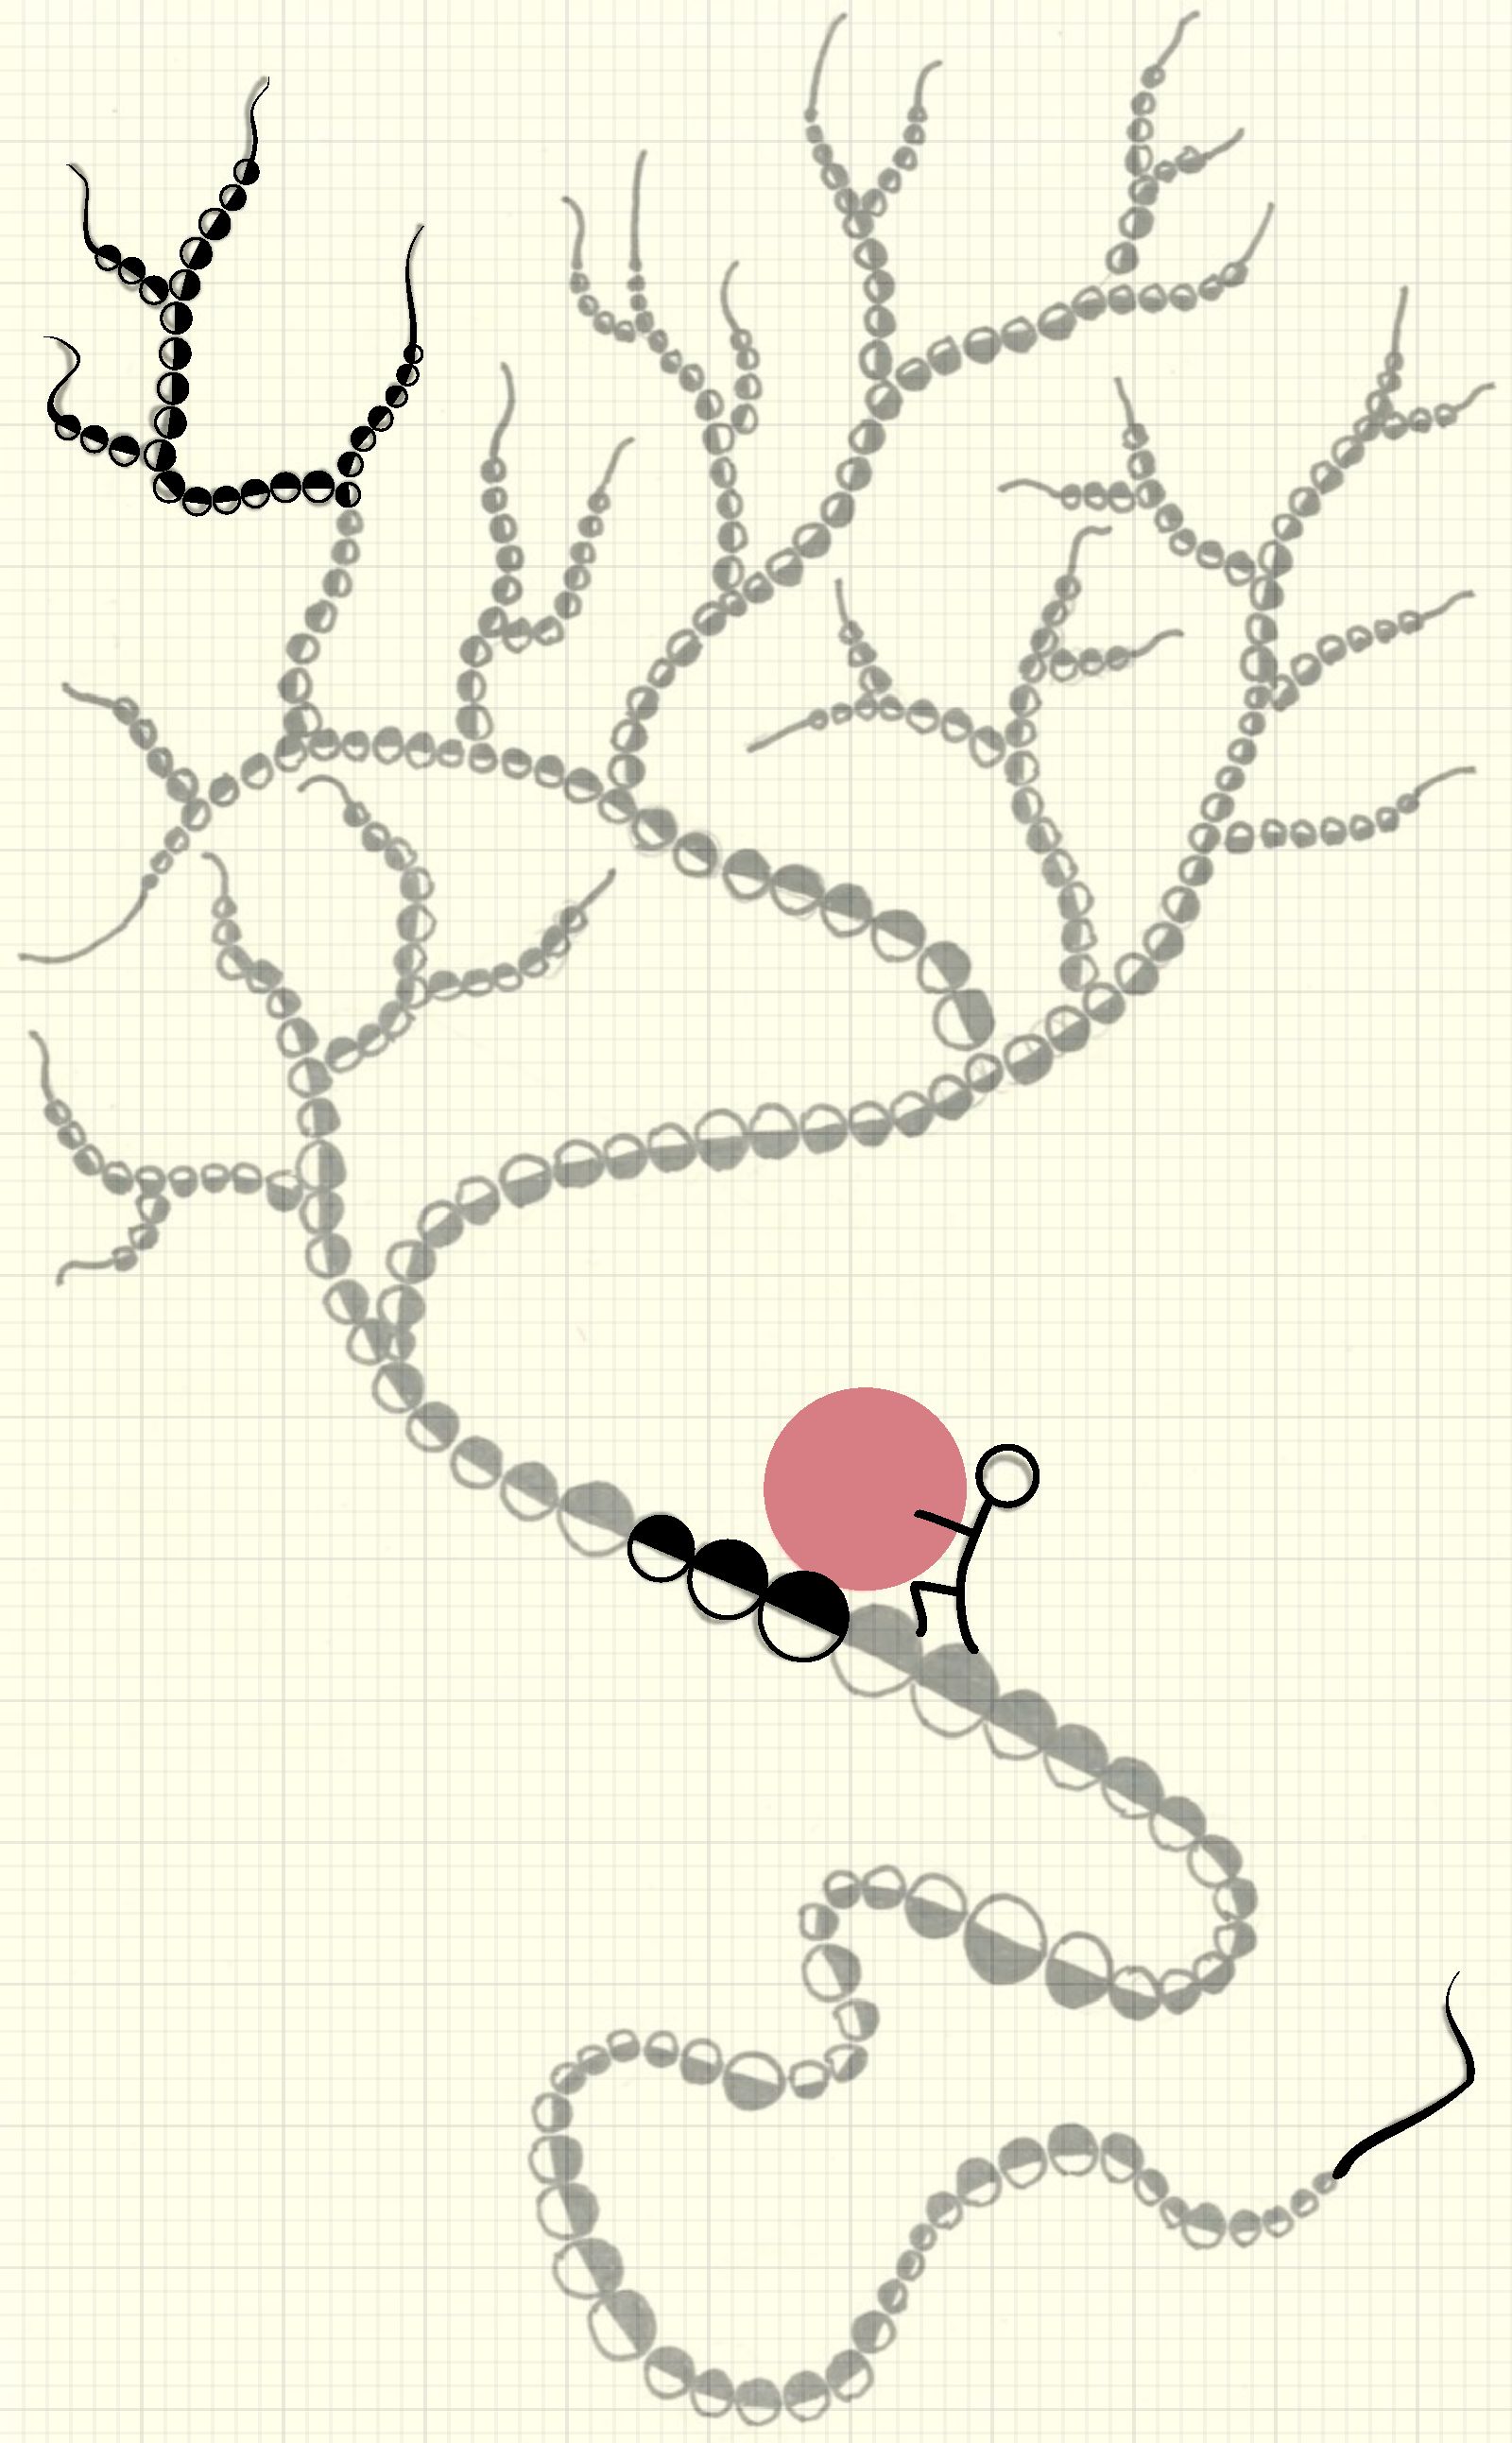
\includegraphics[height=1.15\linewidth]{syziphus}
\end{center}

\begin{textblock*}{\textwidth}(5.8cm,22.4cm)
	{\Huge Miroslav Radojevi\'{c}}
\end{textblock*}

\end{changemargin}

%\clearpage
%\restoregeometry
%}
% ************************************************************************
%
% Cover Page - backside
%
% ************************************************************************
\setlength{\parindent}{0pt}
\thispagestyle{empty}
\newpagecolor{backgroundColor}\afterpage{\restorepagecolor} % so that the color is restored on the following page
\begin{changemargin}{-0.5cm}{-0.5cm}
\end{changemargin}

% ************************************************************************
\end{document}
% ************************************************************************
